\documentclass{beamer}
%\usepackage{beamerarticle}

\usepackage[ngerman]{babel}
\usepackage[utf8]{inputenc}
\usepackage[T1]{fontenc}
\usepackage{tikz}
\usetikzlibrary{positioning, arrows}
\usepackage{listings}
\usepackage{fancybox}

\usetheme{Madrid}
\setbeamercovered{transparent}

\title[SWT-Praktikum]{Pr\"sentationen mit dem Paktet  Beamer}
\author{swp15.gkp}
\date{\today{}}
%\logo{\includegraphics[scale=0.25]{logo}}

\begin{document}
\begin{frame}
\center \huge \textbf{Kartenbasiertes Multiplayerspiel} \\
Pac-Man aka "Pucman"
\end{frame}
\begin{frame}{Überblick}
\begin{itemize}
\item Arbeitsweise
\item Projektvision
\item Vorprojekt
\item Spieldetails
\item Qualitätssicherung
\item Zielsetzung
\end{itemize}
\end{frame}
\begin{frame}
\textbf{Zu uns und unserer Arbeitsweise:}
\begin{itemize}
\item Scum als Vorgehensrahmen
\item verschiedene Rollen je nach individueller Erfahrung
\end{itemize}
\begin{figure}[htb]
  \centering
  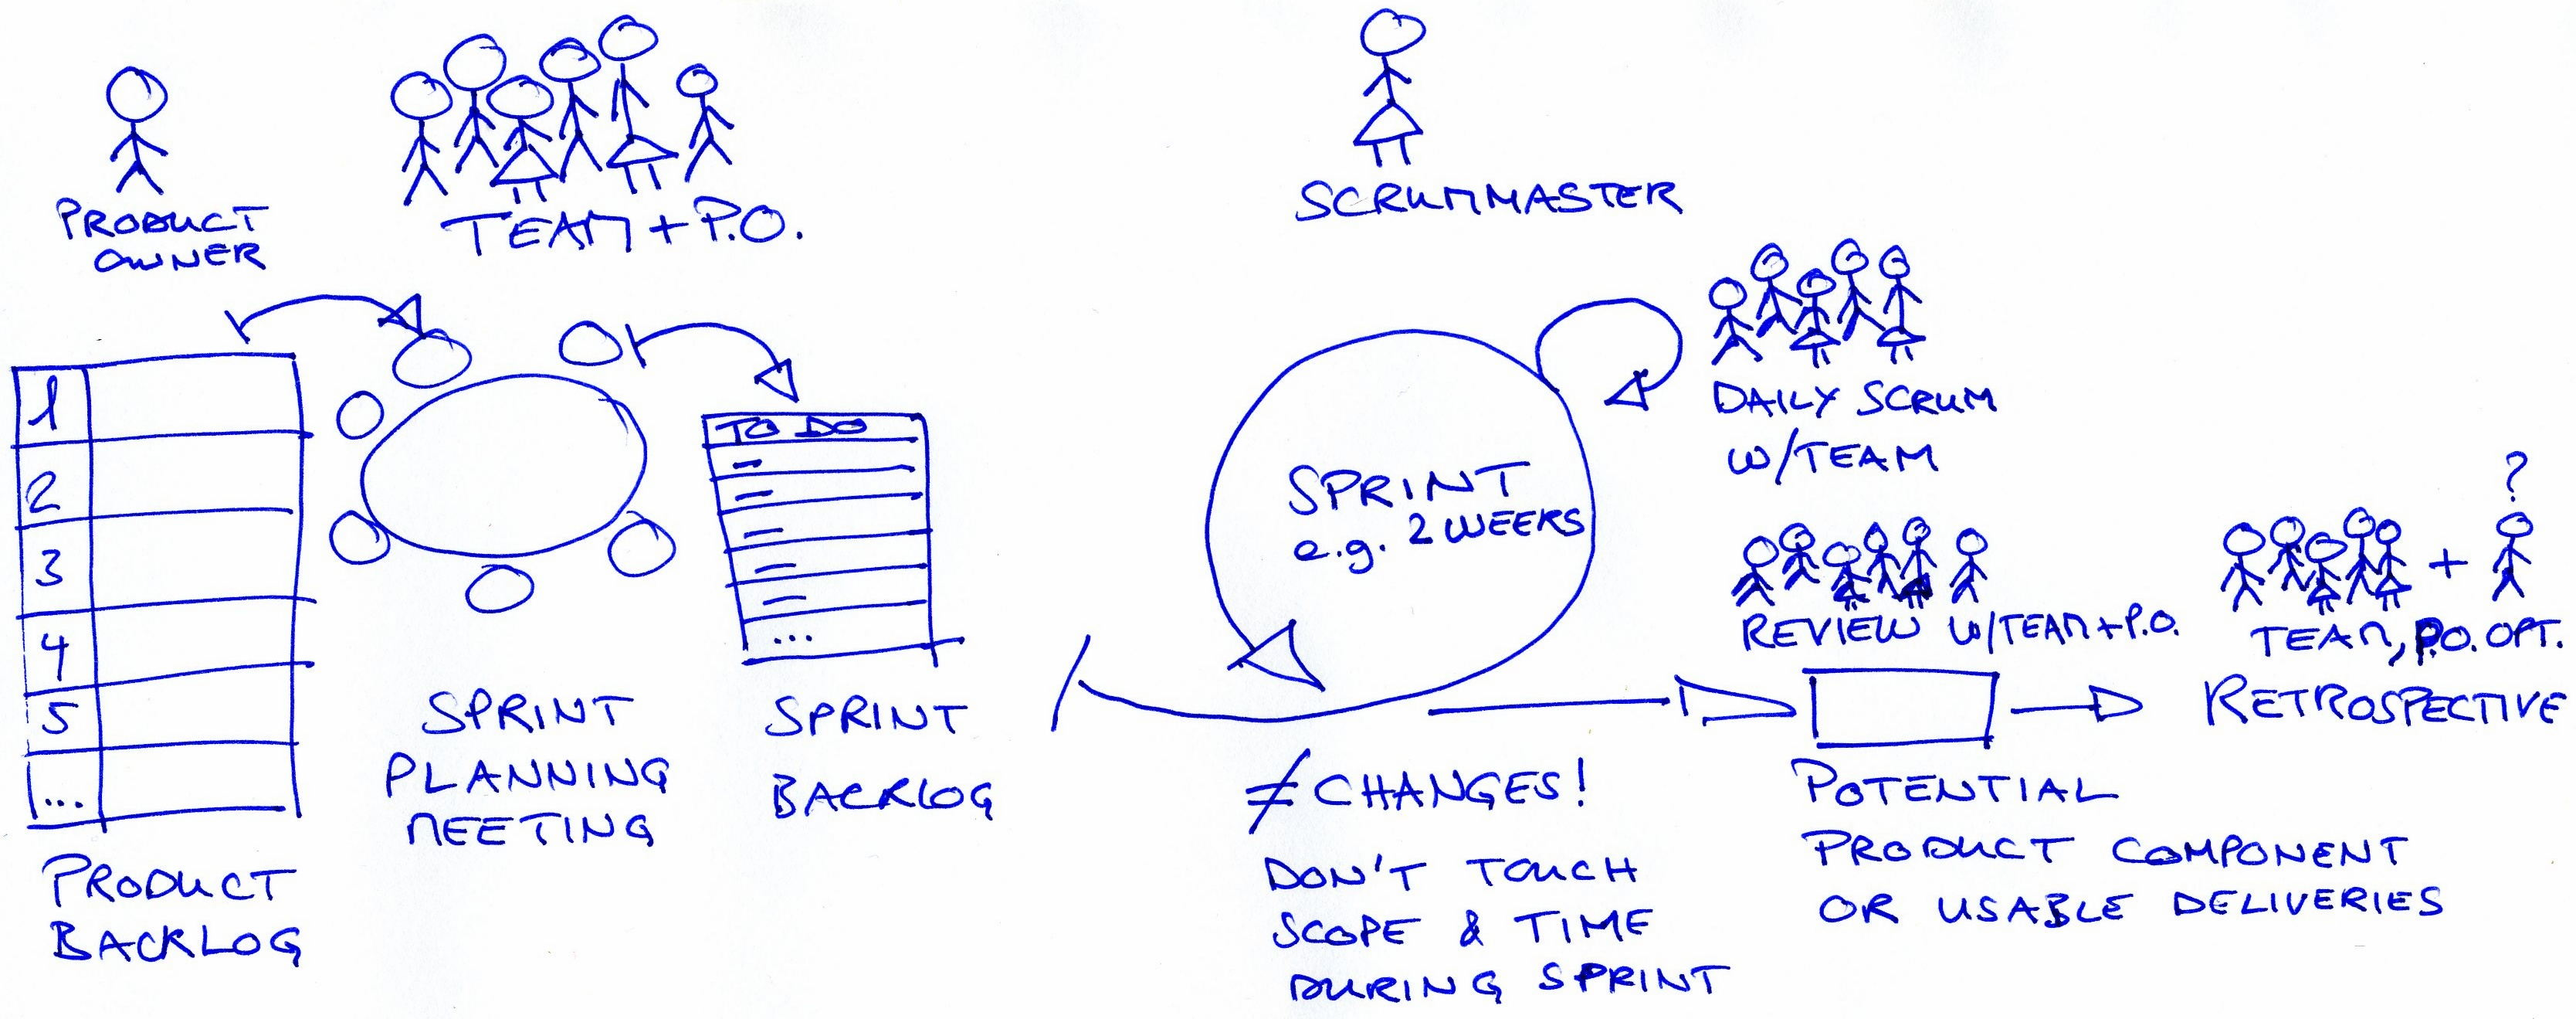
\includegraphics[scale=0.1]{Scrum.jpg}
%\caption{der rote Punkt bezeichnet unser gesuchtes Teilwort}
  \label{PNFs}
\end{figure} 
\end{frame}
\begin{frame}{Projektvision}
\textbf{Was wollen wir erschaffen?}
\begin{itemize}
\item Pac-Man auf einen realen Kartenausschnitt
spielen
\item mit anderen Spielern zusammen spielen
\item Highscores mit denen anderer
vegleichen
\item das ganze als Browsergame
\end{itemize}
\end{frame}
\begin{frame}{Projektvision}
\begin{figure}[htb]
  \centering
  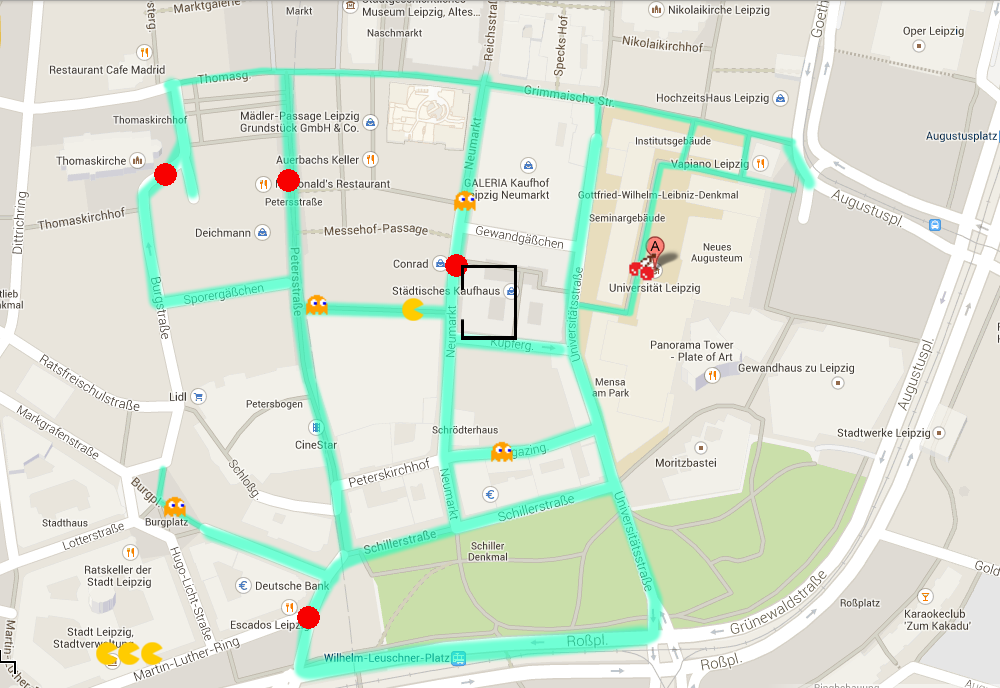
\includegraphics[scale=0.3]{pacman.png}
%\caption{der rote Punkt bezeichnet unser gesuchtes Teilwort}
  \label{PNFs}
\end{figure} 
\end{frame}
\begin{frame}{Funktionalität}
\textbf{Komponenten der Webapplikation}
\begin{itemize}
\item Spielelogik
\item ein
Datenbanksystem zum Speichern der Highscores etc. 
\item ein Kartenmodul
\item ein Layer auf dem Kartenmodul auf dem das Spiel stattfindet
\end{itemize}
\end{frame}
\begin{frame}{Spielelogik}
Die Spielfigur Pac-Man muss Punkte in einem Labyrinth fressen, während sie von Gespenstern verfolgt wird.
\begin{itemize}
\item Frisst man eine „Kraftpille“, kann man für eine gewisse Zeit umgekehrt selbst die (nun blau eingefärbten) Gespenster verfolgen.
\item Manchmal erscheint auch eine Kirsche oder ein anderes Symbol im Spielfeld, das dem Spieler Extrapunkte einbringt, wenn man es frisst.
  Wenn man das Symbol nicht frisst, verschwindet es nach einiger Zeit wieder.
  \item Sind alle Punkte gefressen, gelangt man in den nächsten Level. Dieser unterscheidet sich vom vorigen im Wesentlichen nur durch die höhere Spielgeschwindigkeit (in den niedrigeren Leveln auch durch ein verändertes Gegnerverhalten).
\item
Links und rechts am Bildschirm befindet sich ein Tunnel, durch den man gehen und so die Gegner täuschen kann. Die Gespenster bewegen sich nicht zufällig. Jedes hat eine bestimmte Strategie, die den Bewegungen bzw. Eingaben des Spielers folgt.
\end{itemize}
\end{frame}
\begin{frame}{Datenbanksystem}
Wir brauchen eine Datenstruktur zum speichern der Highscores, der Benutzer, evtl. der Kartendaten etc.
\par\bigskip
\textbf{Frage: welches Datenbanksystem ergibt hier Sinn?}
\end{frame}
\begin{frame}{Kartenmodul + Spiellayer}
Hier kommt alles rein was wir zum Anzeigen brauchen:
\begin{itemize}
\item Kartenlayer - mit Realdaten, die aus Openstreetmaps bezogen wurden (entspricht quasi der Aufgabenstellung des Vorprojekts)
\item Spiellayer - hier findet das Spiel statt 
\end{itemize}
\end{frame}
\begin{frame}{Vorprojekt}
\begin{itemize}
\item Webapplikation
\item Ausschnitt der Geo-Karte
\item auf einfachem Niveau mit der Karte zu agieren
\end{itemize}
Die
Ortsanfrage soll dabei über einen selbst erstellten Web-Server geleitet
werden, der entsprechendes Kartenmaterial aus externen Quellen (einer
Geodatenbank) zur Verfügung stellt und die bereits beschriebene
Zeichen-Komponente (später Spiellayer) mittels einer GUI bereit hält.
\end{frame}
\begin{frame}
\center \huge Spieldetails
\end{frame}
\begin{frame}{Spieldetails Interface}
\begin{itemize}
\item ich möchte auswählen wo auf der Welt ich spiele
\item wenn ich auf Start drücke soll das Spiel starten
\item wenn ich Hilfe benötige, sollten relevante Informationen auf Knopfdruck abrufbar sein  
\item ich möchte das Spielgeschehen hören
\end{itemize}
\end{frame}
\begin{frame}{Gamedesign}
\begin{itemize}
\item möglichst nah an dem original Pac-Man
\item Powerups, Coins, Gespenster
\end{itemize}
\end{frame}
\begin{frame}{Highscore}
\begin{itemize}
\item ich möchte sehen wer auf welcher Karte welche Highscore erzielt hat
\item ich möchte mich auf der Seite einloggen um meine Highscores zu loggen
\item ich möchte meine Highscores auf Social Media posten
\end{itemize}
\end{frame}
\begin{frame}{Mapcreation}
\begin{itemize}
\item ich will, dass die Levelerstellung deterministisch abläuft
\item ich möchte an einen beliebigen Ort spielen können
\end{itemize}
\end{frame}
\begin{frame}{Spieldetails}
\begin{block}{Fragen über Fragen}
Was soll passieren wenn ein Ort ausgewäht wurde?
\end{block}
\textbf{Highscore}
\begin{itemize}
\item Automatische, deterministische, eindeutige Kartengenerierung zu bestimmten Orten, z.B. Leipzig, Hamburg, Berlin, mit Highscore.
\item andere Karten möglich, aber nicht mit vergleichbaren Highscores
\item Ähnlichkeit zu der original Pac-Man Karte
\end{itemize}
\begin{figure}[htb]
  \centering
  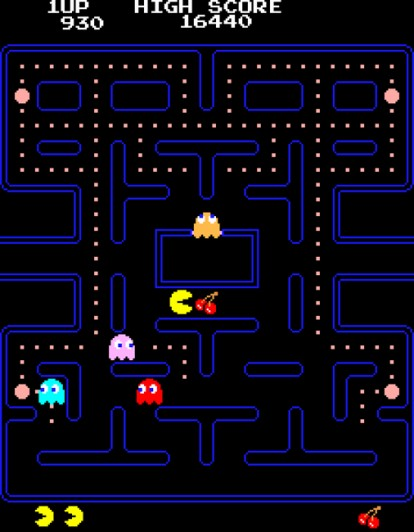
\includegraphics[scale=0.2]{pacman2.jpg}
%\caption{der rote Punkt bezeichnet unser gesuchtes Teilwort}
  \label{PNFs}
\end{figure} 
\end{frame}
\begin{frame}{Stichwort semantic Web}
\textbf{Wie wollen wir die Daten aus dem semantic Web in das Spiel einfließen lassen?}
\begin{itemize}
\item öffentliche Gebäude $\rightarrow$ an der Polizeistation spawnen die Geister, Powerups an Krankenhäusern
\item Tempolimit für die Geister?
\item Idee: Pokemon Datenbank, Pokemon als Geister $\rightarrow$ z.B. elektro Pkmn sind schneller in der Nähe von Kraftwerken etc. 
\end{itemize}
\end{frame}
\begin{frame}{Qualitätssicherung}
\textbf{Unsere Qualitätsstandards:}
\begin{itemize}
\item Programmierstandards - Sun-Java-Codeconventions von 1997
\item Quelltextdokumentation
\item Testkonzepte - fehlerfreier Code durch	 JUnit, JSUnit
\end{itemize}
\par\bigskip	
\textbf{Eine
gute Dokumentation verkürzt die Einarbeitungszeit projektfremder
Entwickler in den Quellcode und erleichtert damit die Wartung und
Weiterentwicklung der Software.}

\end{frame}
\begin{frame}{Das angestrebte Ziel}
\center  \textbf{Das Spiel soll zu 100\% lauffähig sein!}
\end{frame}
\begin{frame}
\center  \textbf{noch Fragen?}
\par\bigskip
\center  \textbf{Vielen Dank für die Aufmerksamkeit}

\end{frame}
\end{document}